\section{Справочные сведения о походе} 
\subsection{Проводящая организация}
Поход был совершён в рамках школы горного туризма базового уровня, организованной Горной секцией МФТИ.


\subsection{Место проведения}
\textbf{Страна:} Россия

\textbf{Субъекты федерации:} КЧР, КБР

\textbf{Район:} Западный Кавказ

\textbf{Подрайоны:} Гвандра, Приэльбрусье

\subsection{Общие справочные сведения о маршруте}

\begin{table}[h!]
	\resizebox{\textwidth}{!}{%
		\begin{tabular}{|c|c|c|cc|c|}
			\hline
			\multirow{2}{*}{\begin{tabular}[c]{@{}c@{}}Дисциплина\\ (вид туризма)\end{tabular}} & \multirow{2}{*}{\begin{tabular}[c]{@{}c@{}}Категория сложности\\ маршрута\end{tabular}} & \multirow{2}{*}{\begin{tabular}[c]{@{}c@{}}Протяжённость\\ активной части, км$^1$\end{tabular}} & \multicolumn{2}{c|}{\begin{tabular}[c]{@{}c@{}}Продолжительность активной\\ части\end{tabular}} & \multirow{2}{*}{Сроки проведения}                                   \\ \cline{4-5}
			&                                                                                         &                                                                                             & \multicolumn{1}{c|}{Общая}                            & Ходовых дней                            &                                                                     \\ \hline
			Горный                                                                              & Первая                                                                                  & 111.0                                                                                         & \multicolumn{1}{c|}{13}                               & 13                                      & \begin{tabular}[c]{@{}c@{}}18.08.2024~--\\ 30.08.2024 г.\end{tabular} \\ \hline
		\end{tabular}%
	}
\end{table}
\footnotesize{$^1$ С учётом коэффициента $k=1.2$, без учёта повторно пройденного пути}
\normalsize

\subsection{Подробная нитка маршрута}
\textbf{Заявленная:} г. Минеральные Воды~--- д.р. Учкулан~--- д.р. Кичкинакол Уллукёльский~--- \textbf{пер. Уллукёль Восточный (1А, 3050)}~--- т/б <<Глобус>>~--- д.р.Гондарай~--- д.р. Джалпаккол~--- \textbf{пер. Джалпаккол Северный (1А, 3400)}~--- д.р. Мырды~--- а/л<<Узункол>>~--- д.р.Кичкинекол~--- д.р. Таллычат~--- \textbf{пер. Кичкинекол Малый (1А, 3210)}~--- д.р. Чунгур-Джар~--- \textbf{пер. Перемётный (1А, 3242)}~--- д.р. Танышхан~--- д.р. Чиринкол~--- стоянка <<Гвандра>>~--- д. р. Кубань~--- \textbf{пер. Хотютау (1А, 3546)}~--- лед. Большой Азау~--- ст. <<Кругозор>>.

\textbf{Пройденная:} Маршрут пройден без изменений.

\textbf{Корнилов Георгий} сошёл с маршрута в т/б <<Глобус>>. Он прошёл перевал Уллукёль Восточный (1А$^{\star}$). Пройдено расстояние $L=25.1~\text{км}$ за 4 ходовых дня.

\textbf{Миронова Наталья} сошла с маршрута в а/л <<Узункол>>. Она прошла перевалы Уллукёль Восточный (1А$^{\star}$), Джалпаккол Северный (1А$^{\star}$). Пройдено расстояние $L=48.
1~\text{км}$ за 7 ходовых дней.

\textbf{Шалфеев Илья, Мерзликина Дарья, Сингалевич Дмитрий, Семено Мария} сошли с маршрута после д.р. Чиринкол, на погранзаставе <<Хурзук>>. Они прошли перевалы Уллукёль Восточный (1А$^{\star}$), Джалпаккол Северный (1А$^{\star}$), Кичкинекол Малый (1А), Перемётный (1А). Пройдено расстояние $L=85.
7~\text{км}$ за 11 ходовых дней.

\begin{figure}[h!tbp]
	\centering
	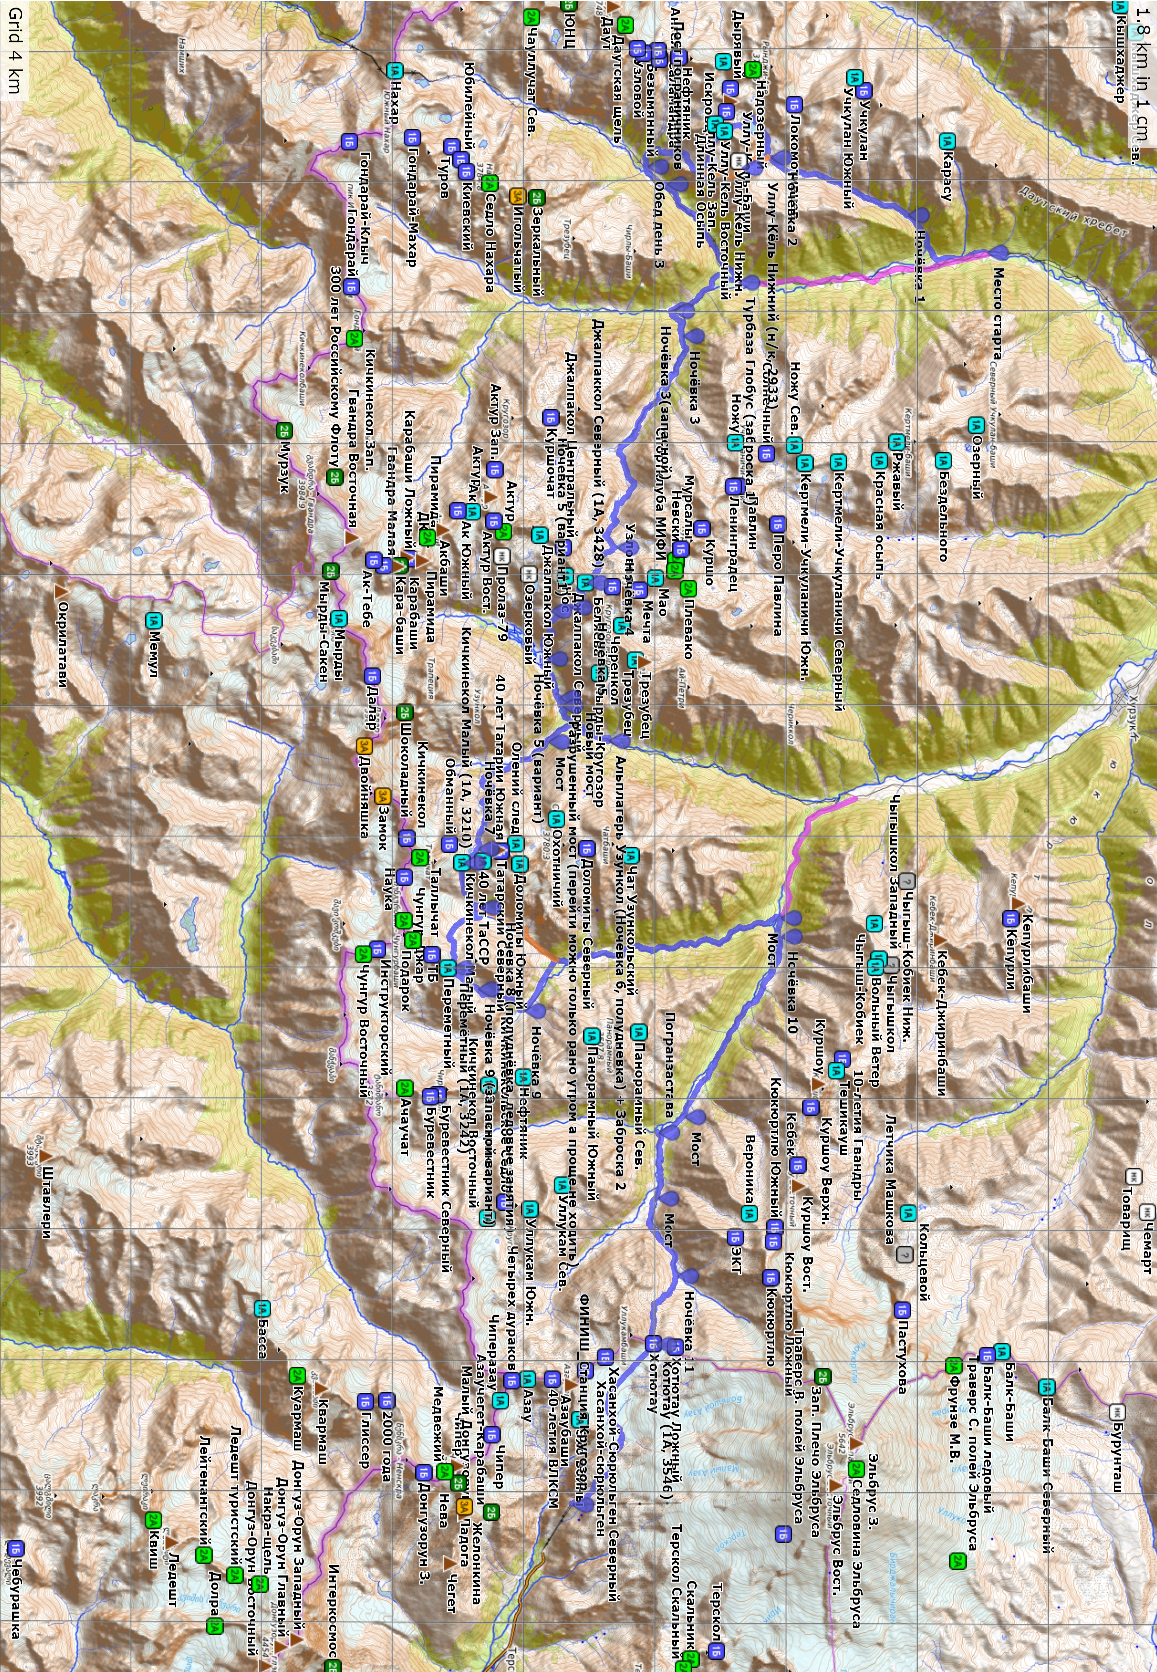
\includegraphics[width=0.92\linewidth]{../pics/map}
	\caption{Обзорная схема маршрута}
\end{figure}

\newpage
\subsection{Высотный профиль маршрута}

\begin{figure}[h!]
	\centering
	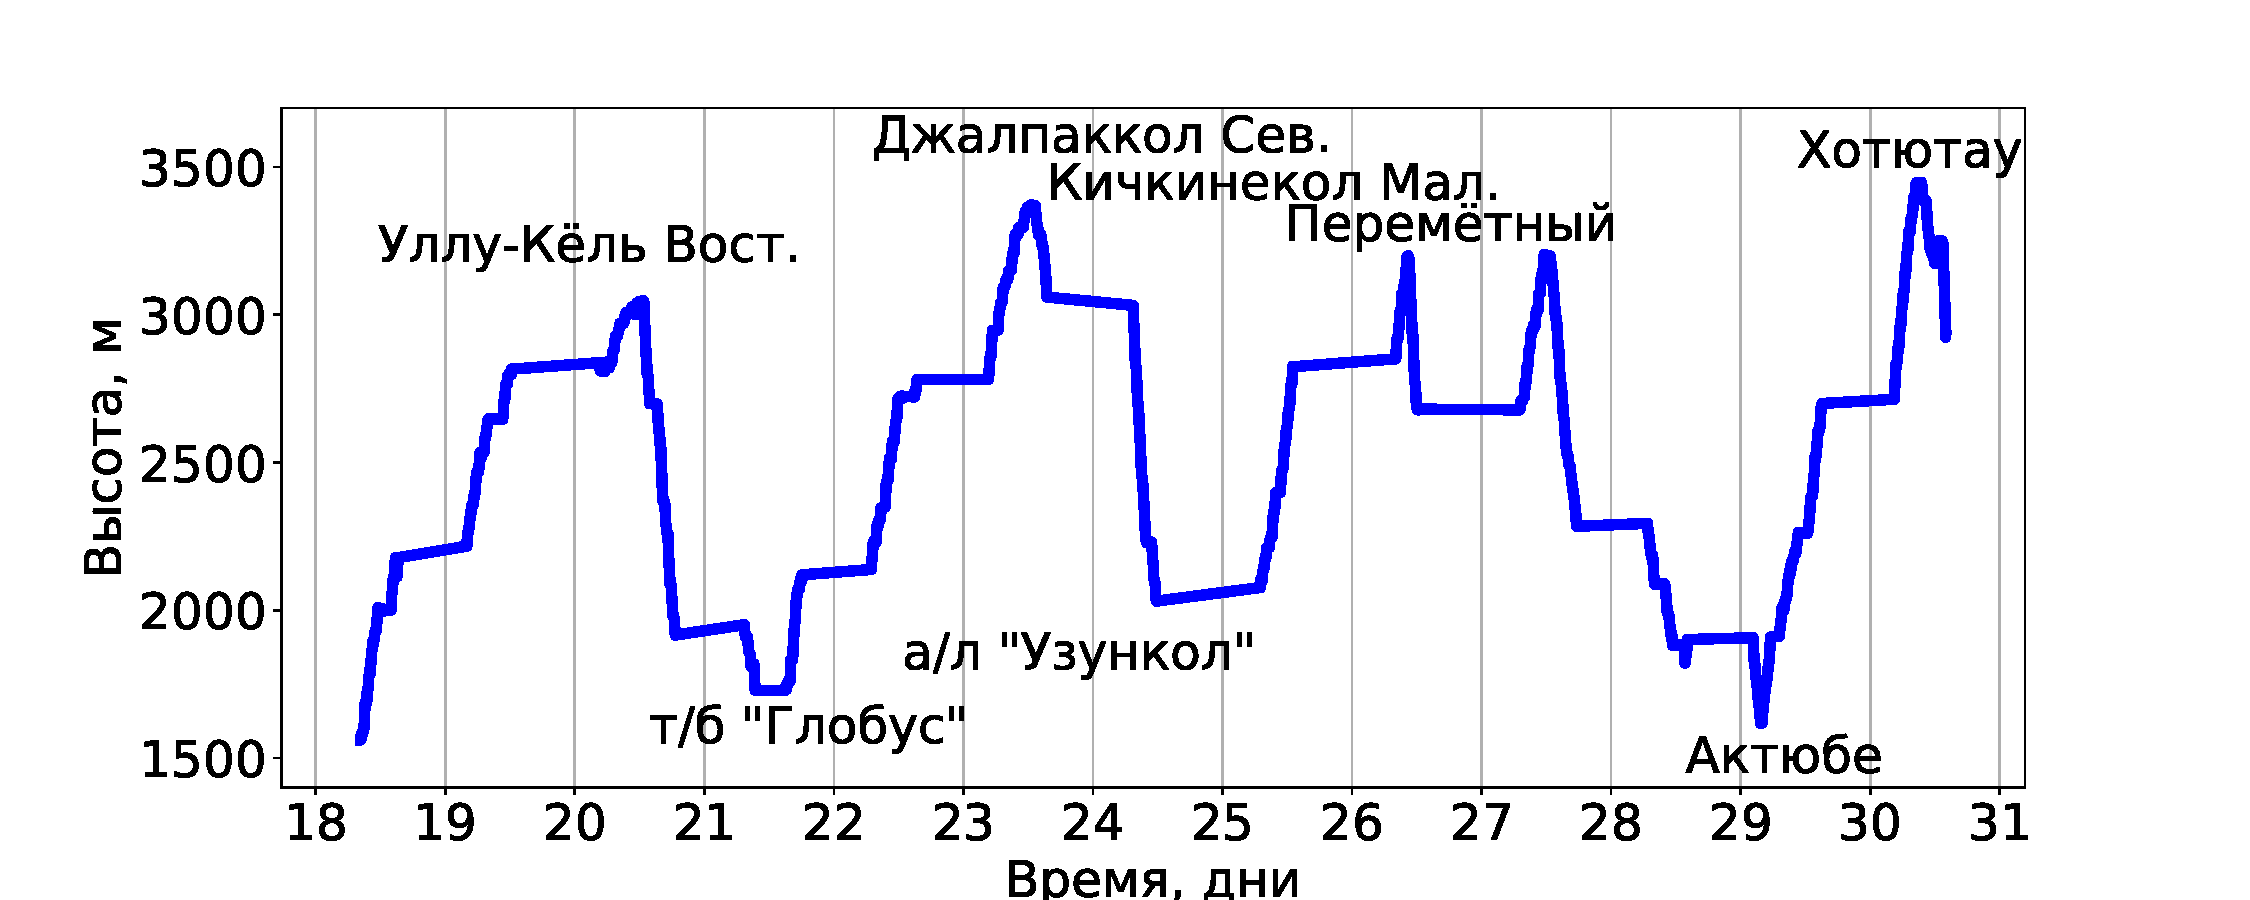
\includegraphics[width=0.92\linewidth]{../pics/elevation_vs_time}
	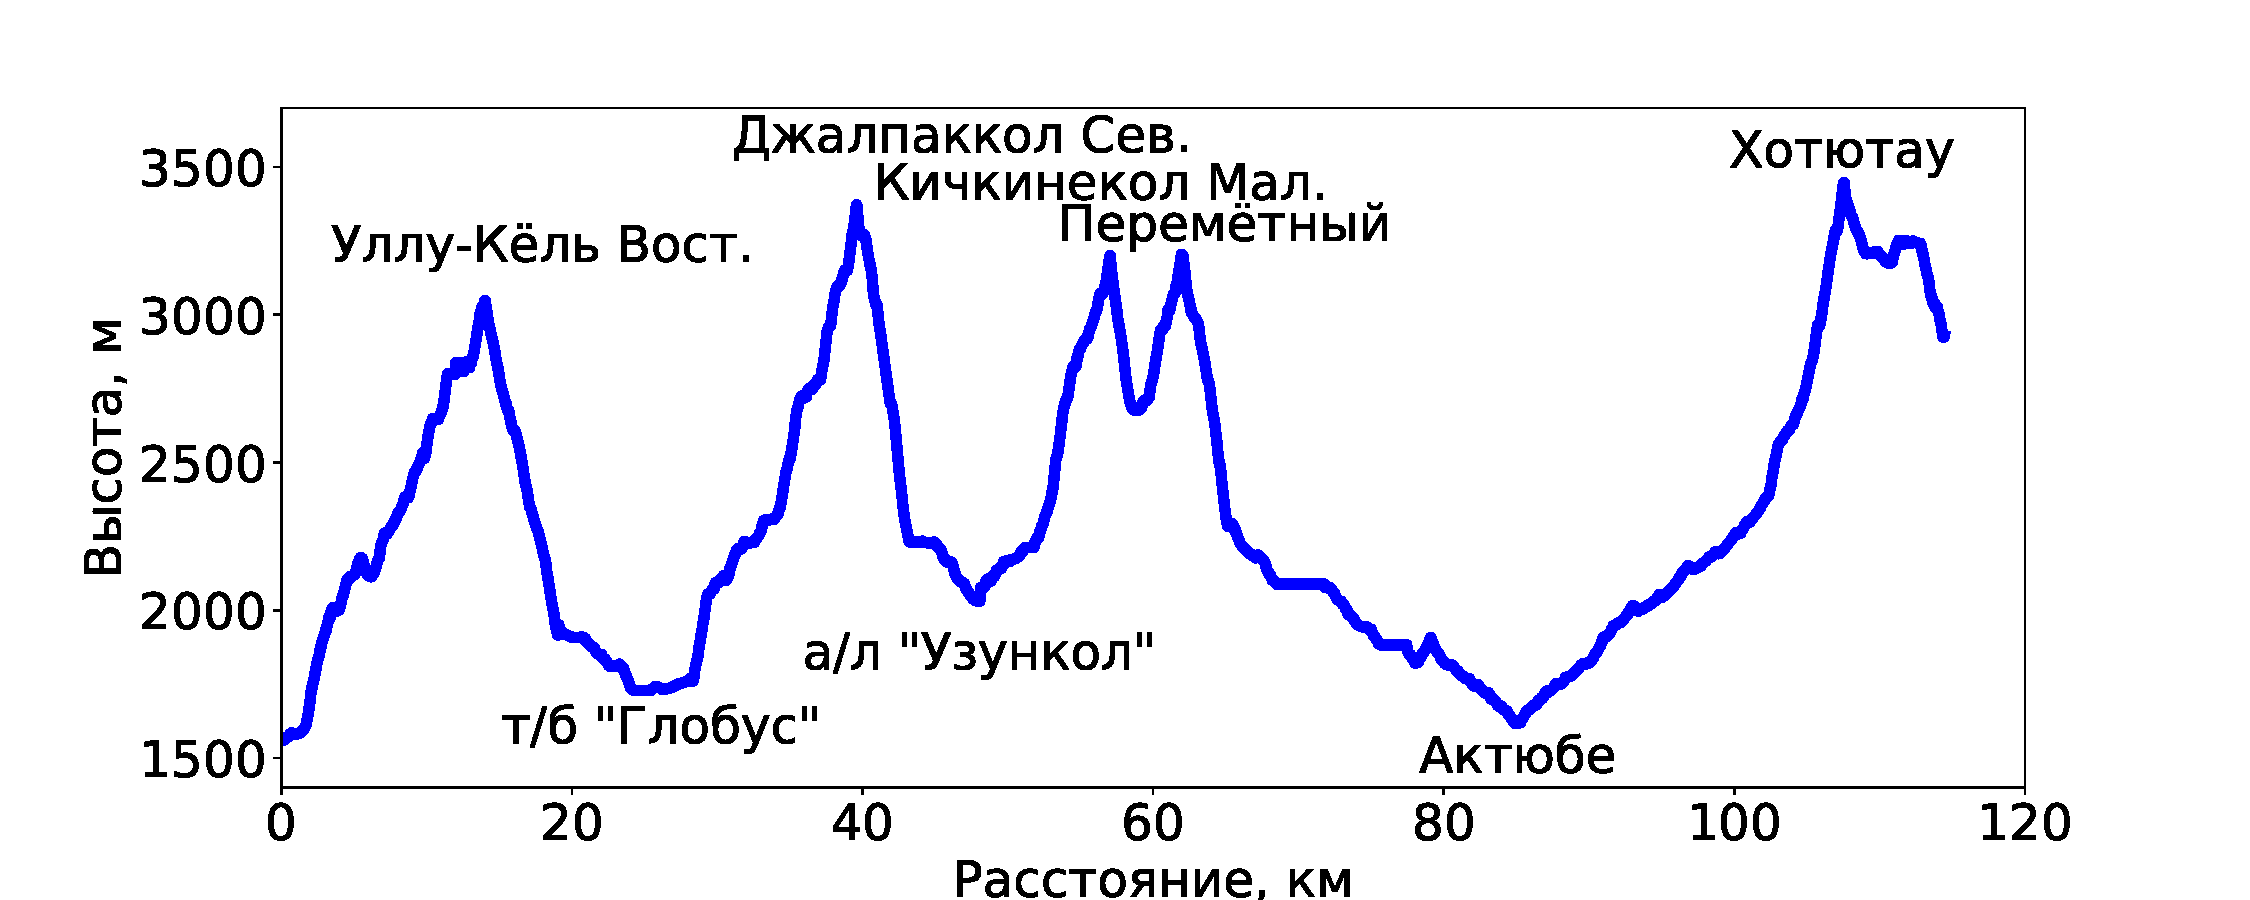
\includegraphics[width=0.92\linewidth]{../pics/elevation_vs_distance}
	\caption{Высотный профиль маршрута}
	\label{fig:heights}
\end{figure}

\newpage
\subsection{Определяющие препятствия маршрута}

\begin{table}[h!]
		\begin{tabular}{|>{\centering\arraybackslash}m{0.17\linewidth}|>{\centering\arraybackslash}m{0.03\linewidth}|>{\centering\arraybackslash}m{0.4\linewidth}|>{\centering\arraybackslash}m{0.3\linewidth}|}
			\hline
			\textbf{Вид препятствия, высота} &
			\begin{turn}{90}\textbf{к. тр.}\end{turn} &
			\textbf{Характеристика препятствия на подъём} &
			\textbf{Характеристика препятствия на спуск} \\
			\hline			
			пер. Уллу-Кёль Восточный, 3050 & 1А$^{\star}$ &  Со стороны оз. Уллукёль ск.-сн.-ос. перевальный взлёт протяжённостью до 350 м. У подножия крутизна $20-25^{\circ}$; далее осыпной участок крутизной до $30^{\circ}$ протяжённостью до 100 м и далее снежник крутизной до $35-40^{\circ}$, а в верхней части до $45^{\circ}$, протяжённостью до 50 м. & Движение по гребню до озера под перевалом, далее травяной склон \\
			\hline			
			пер. Джалпаккол Северный, 3411  & 1А$^{\star}$ & Со стороны д.р. Джалпаккол перевальный взлёт лед.-ос. протяжённостью до 200 м, крутизной $35-40^{\circ}$. Выход на перевал — 5 м простого лазания на скальный гребень.  & ск.-ос., протяжённостью до 150 м, крутизной до $30^{\circ}$ \\
			\hline
			пер. Кичкинекол Малый, 3206  & 1А & Со стороны д.р. Кичкинекол по тр.-ос. склону по тропе, протяжённостью до 300 м, крутизной до $25^{\circ}$. На седловине перевала снежник. & ск.-ос. тропа протяжённостью до 200 м., крутизной до $15^{\circ}$\\
			\hline
			пер. Перемётный, 3255  & 1А & Со стороны д.р. Чунгур-Джар перевальный взлёт ск.-ос. протяжённостью до 400 м, крутизной до  $20^{\circ}$ & ск.-ос. склон протяжённостью до 100 м, крутизной до $35^{\circ}$, далее косым траверсом по курумнику. Обход сбросов левее березняка по лощине.\\
			\hline
			пер. Хотютау, 3546  & 1А$^{\star}$ & Со стороны д.р. Уллу-Кам подъём по ос.склону протяжённостью до 1000 м, крутизной до $25^{\circ}$. &  ос. склон протяжённостью до 70 м, крутизной до $30^{\circ}$, выход на открытый ледник\\
			\hline
	\end{tabular}%
\end{table}

\newpage
\subsection{Список участников} 

\begin{table}[h!]
	\centering
	\resizebox{0.7\textwidth}{!}{%
	\begin{tabular}{|>{\centering\arraybackslash}m{0.02\linewidth}|>{\centering\arraybackslash}m{0.2\linewidth}|>{\centering\arraybackslash}m{0.14\linewidth}|>{\centering\arraybackslash}m{0.05\linewidth}|>{\centering\arraybackslash}m{0.15\linewidth}|>{\centering\arraybackslash}m{0.18\linewidth}|}
		\hline
		\textbf{№} &
		\textbf{Фото} &
		\textbf{ФИО} &
		\textbf{г.р.} &
		\textbf{Обязанности в группе} &
		\textbf{Спортивный опыт} \\
		\hline			
		
		1	&	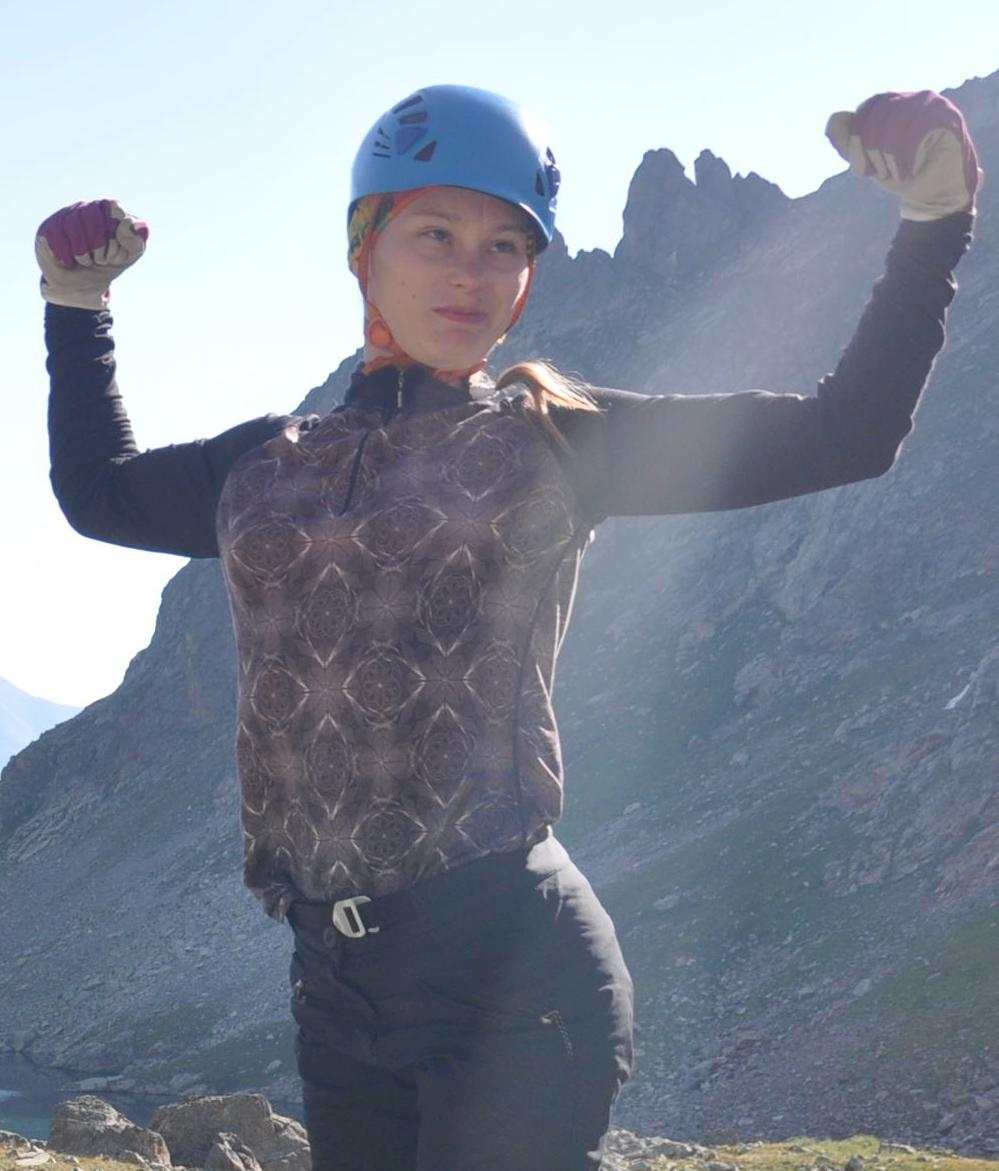
\includegraphics[width=0.99\linewidth]{../pics/portraits/dasha_s}	&	Снеговская Дарья Алексеевна	&	1997	&	Руководитель	& 3ГУ, Центральный Кавказ, 2020 \newline 1ГУ, Алтай, Северо-Чуйский хребет, 2023 \\
		\hline
		2	& 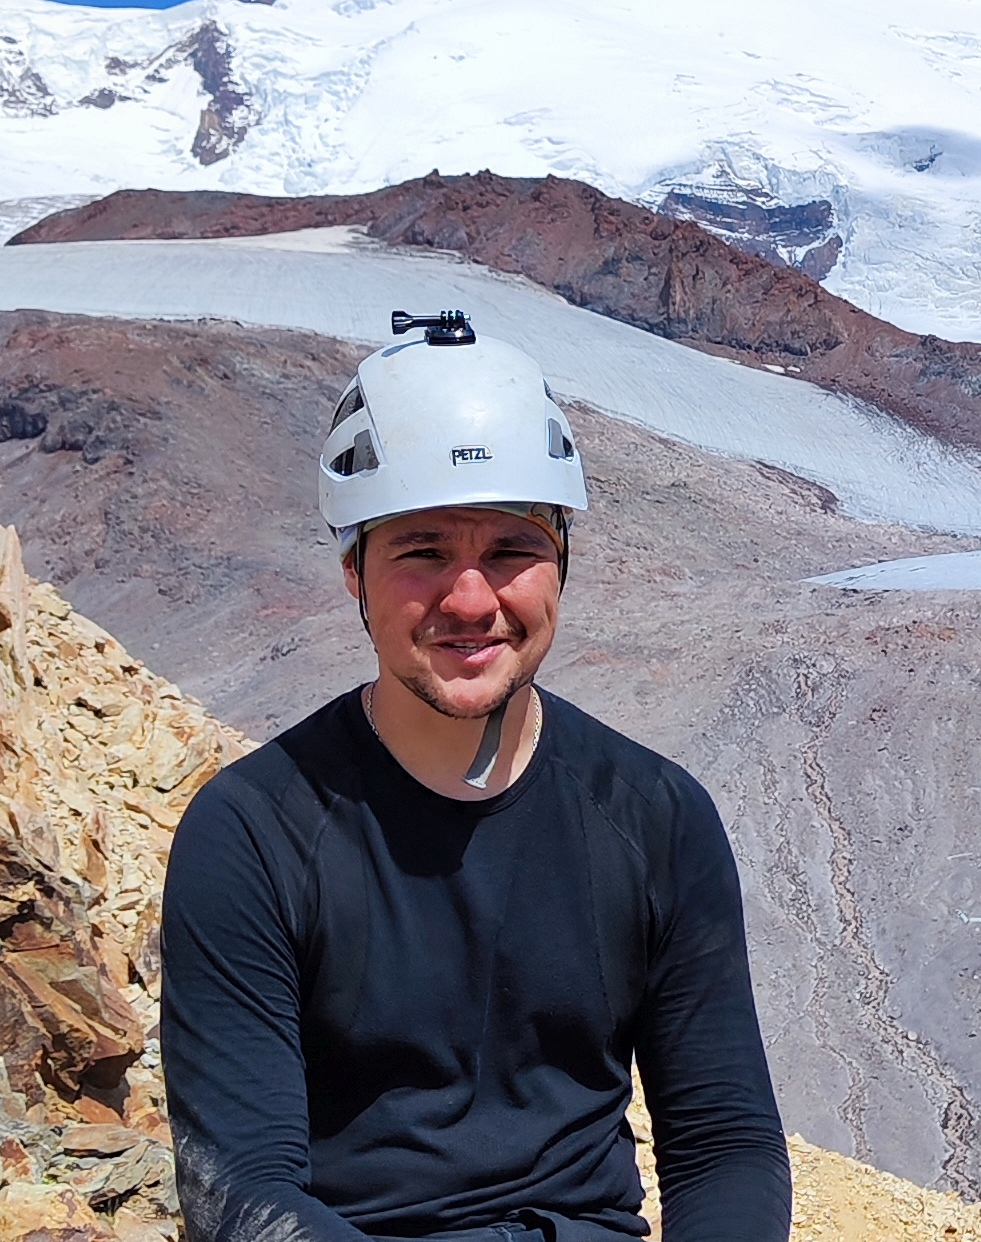
\includegraphics[width=0.99\linewidth]{../pics/portraits/lesha_o1}	&	Остапив Алексей Юрьевич	&	1998	&	Зам. руководителя	& 2ГУ, Киргизский хребет, 2019 \newline 1ГУ, Алтай, Северо-Чуйский хребет, 2023 \\
		\hline
		3	&	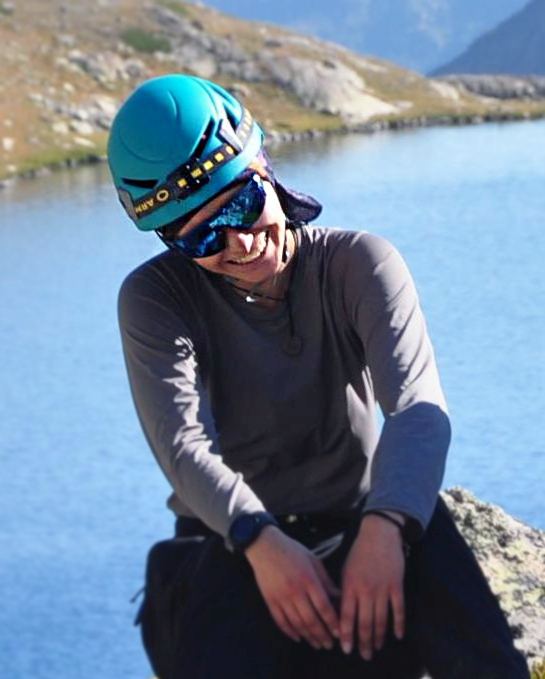
\includegraphics[width=0.99\linewidth]{../pics/portraits/katya}	&	Тюрина Екатерина Алексеевна	&	2004	&	Медик	&	1 ст.с. \\
		\hline
		4	&		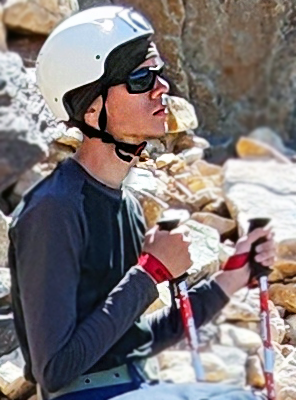
\includegraphics[width=0.99\linewidth]{../pics/portraits/dima_d}		&	Дёмушкин .Дмитрий Юрьевич	&	2001	&	Штурман	&	1 ст.с. \\
		\hline
		5	&	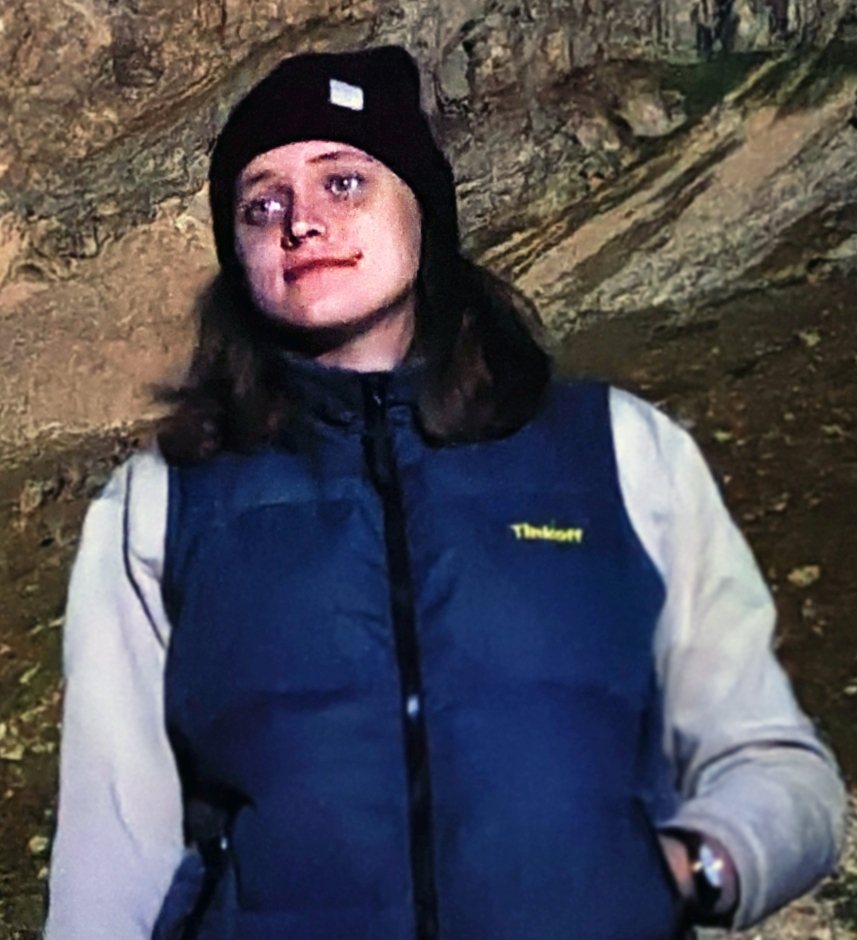
\includegraphics[width=0.99\linewidth]{../pics/portraits/natasha}	&	Миронова Наталья Сергеевна	&	2000	&	Хронометрист	&	1 ст.с. \\
		\hline
		6	&	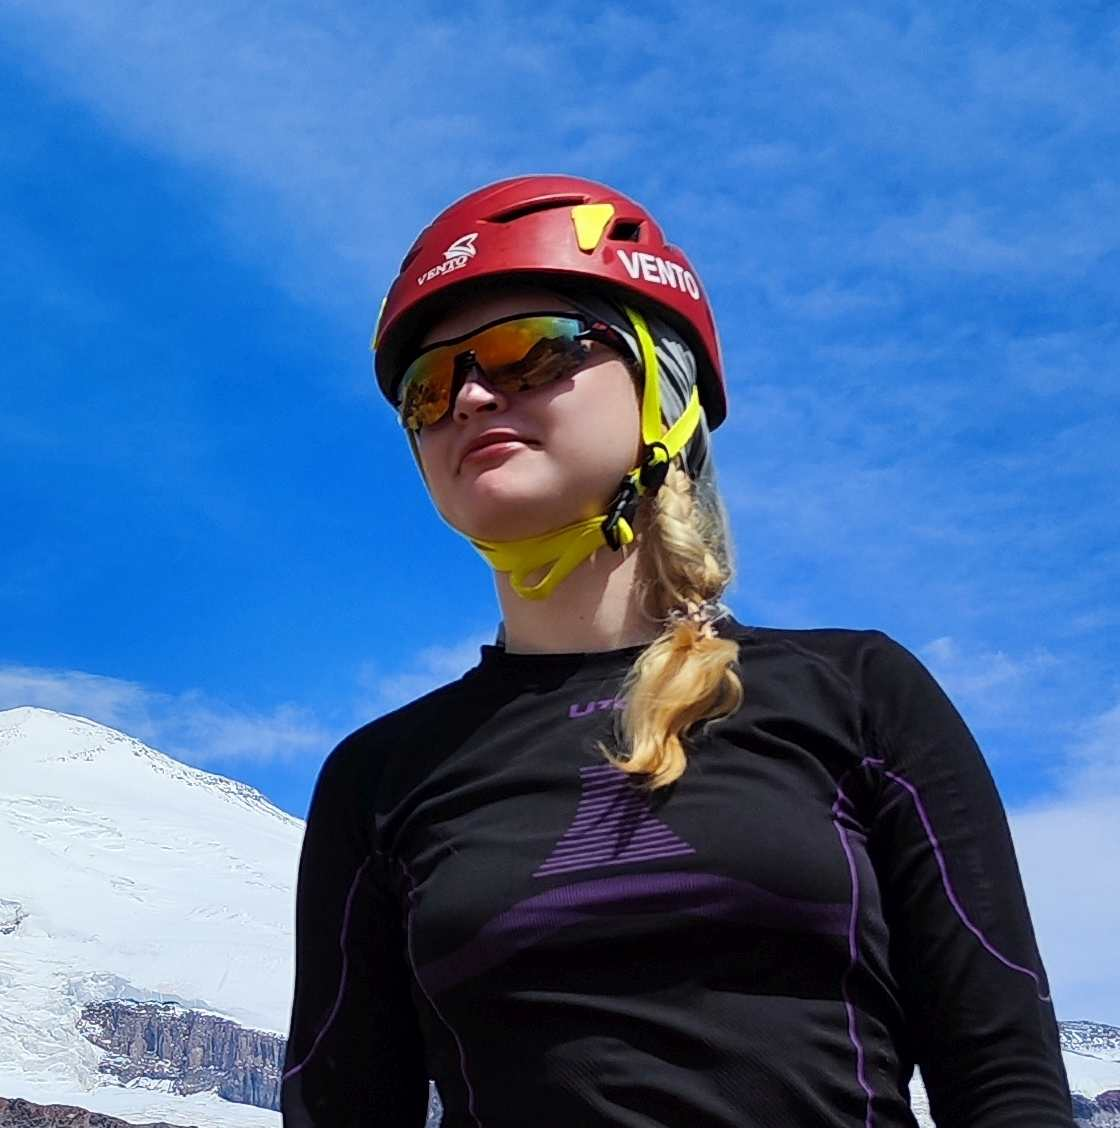
\includegraphics[width=0.99\linewidth]{../pics/portraits/dasha_k}	&	Казаринова Дарья Дмитриевна	&	2001	&	Логист	&	1 ст.с. \\
	\hline
	\end{tabular}%
	}
\end{table}

\newpage

\begin{table}[h!]
	\centering
	\resizebox{0.7\textwidth}{!}{%
	\begin{tabular}{|>{\centering\arraybackslash}m{0.02\linewidth}|>{\centering\arraybackslash}m{0.2\linewidth}|>{\centering\arraybackslash}m{0.14\linewidth}|>{\centering\arraybackslash}m{0.05\linewidth}|>{\centering\arraybackslash}m{0.15\linewidth}|>{\centering\arraybackslash}m{0.18\linewidth}|}
		\hline
		\textbf{№} &
		\textbf{Фото} &
		\textbf{ФИО} &
		\textbf{г.р.} &
		\textbf{Обязанности в группе} &
		\textbf{Спортивный опыт} \\
		\hline
		7	&	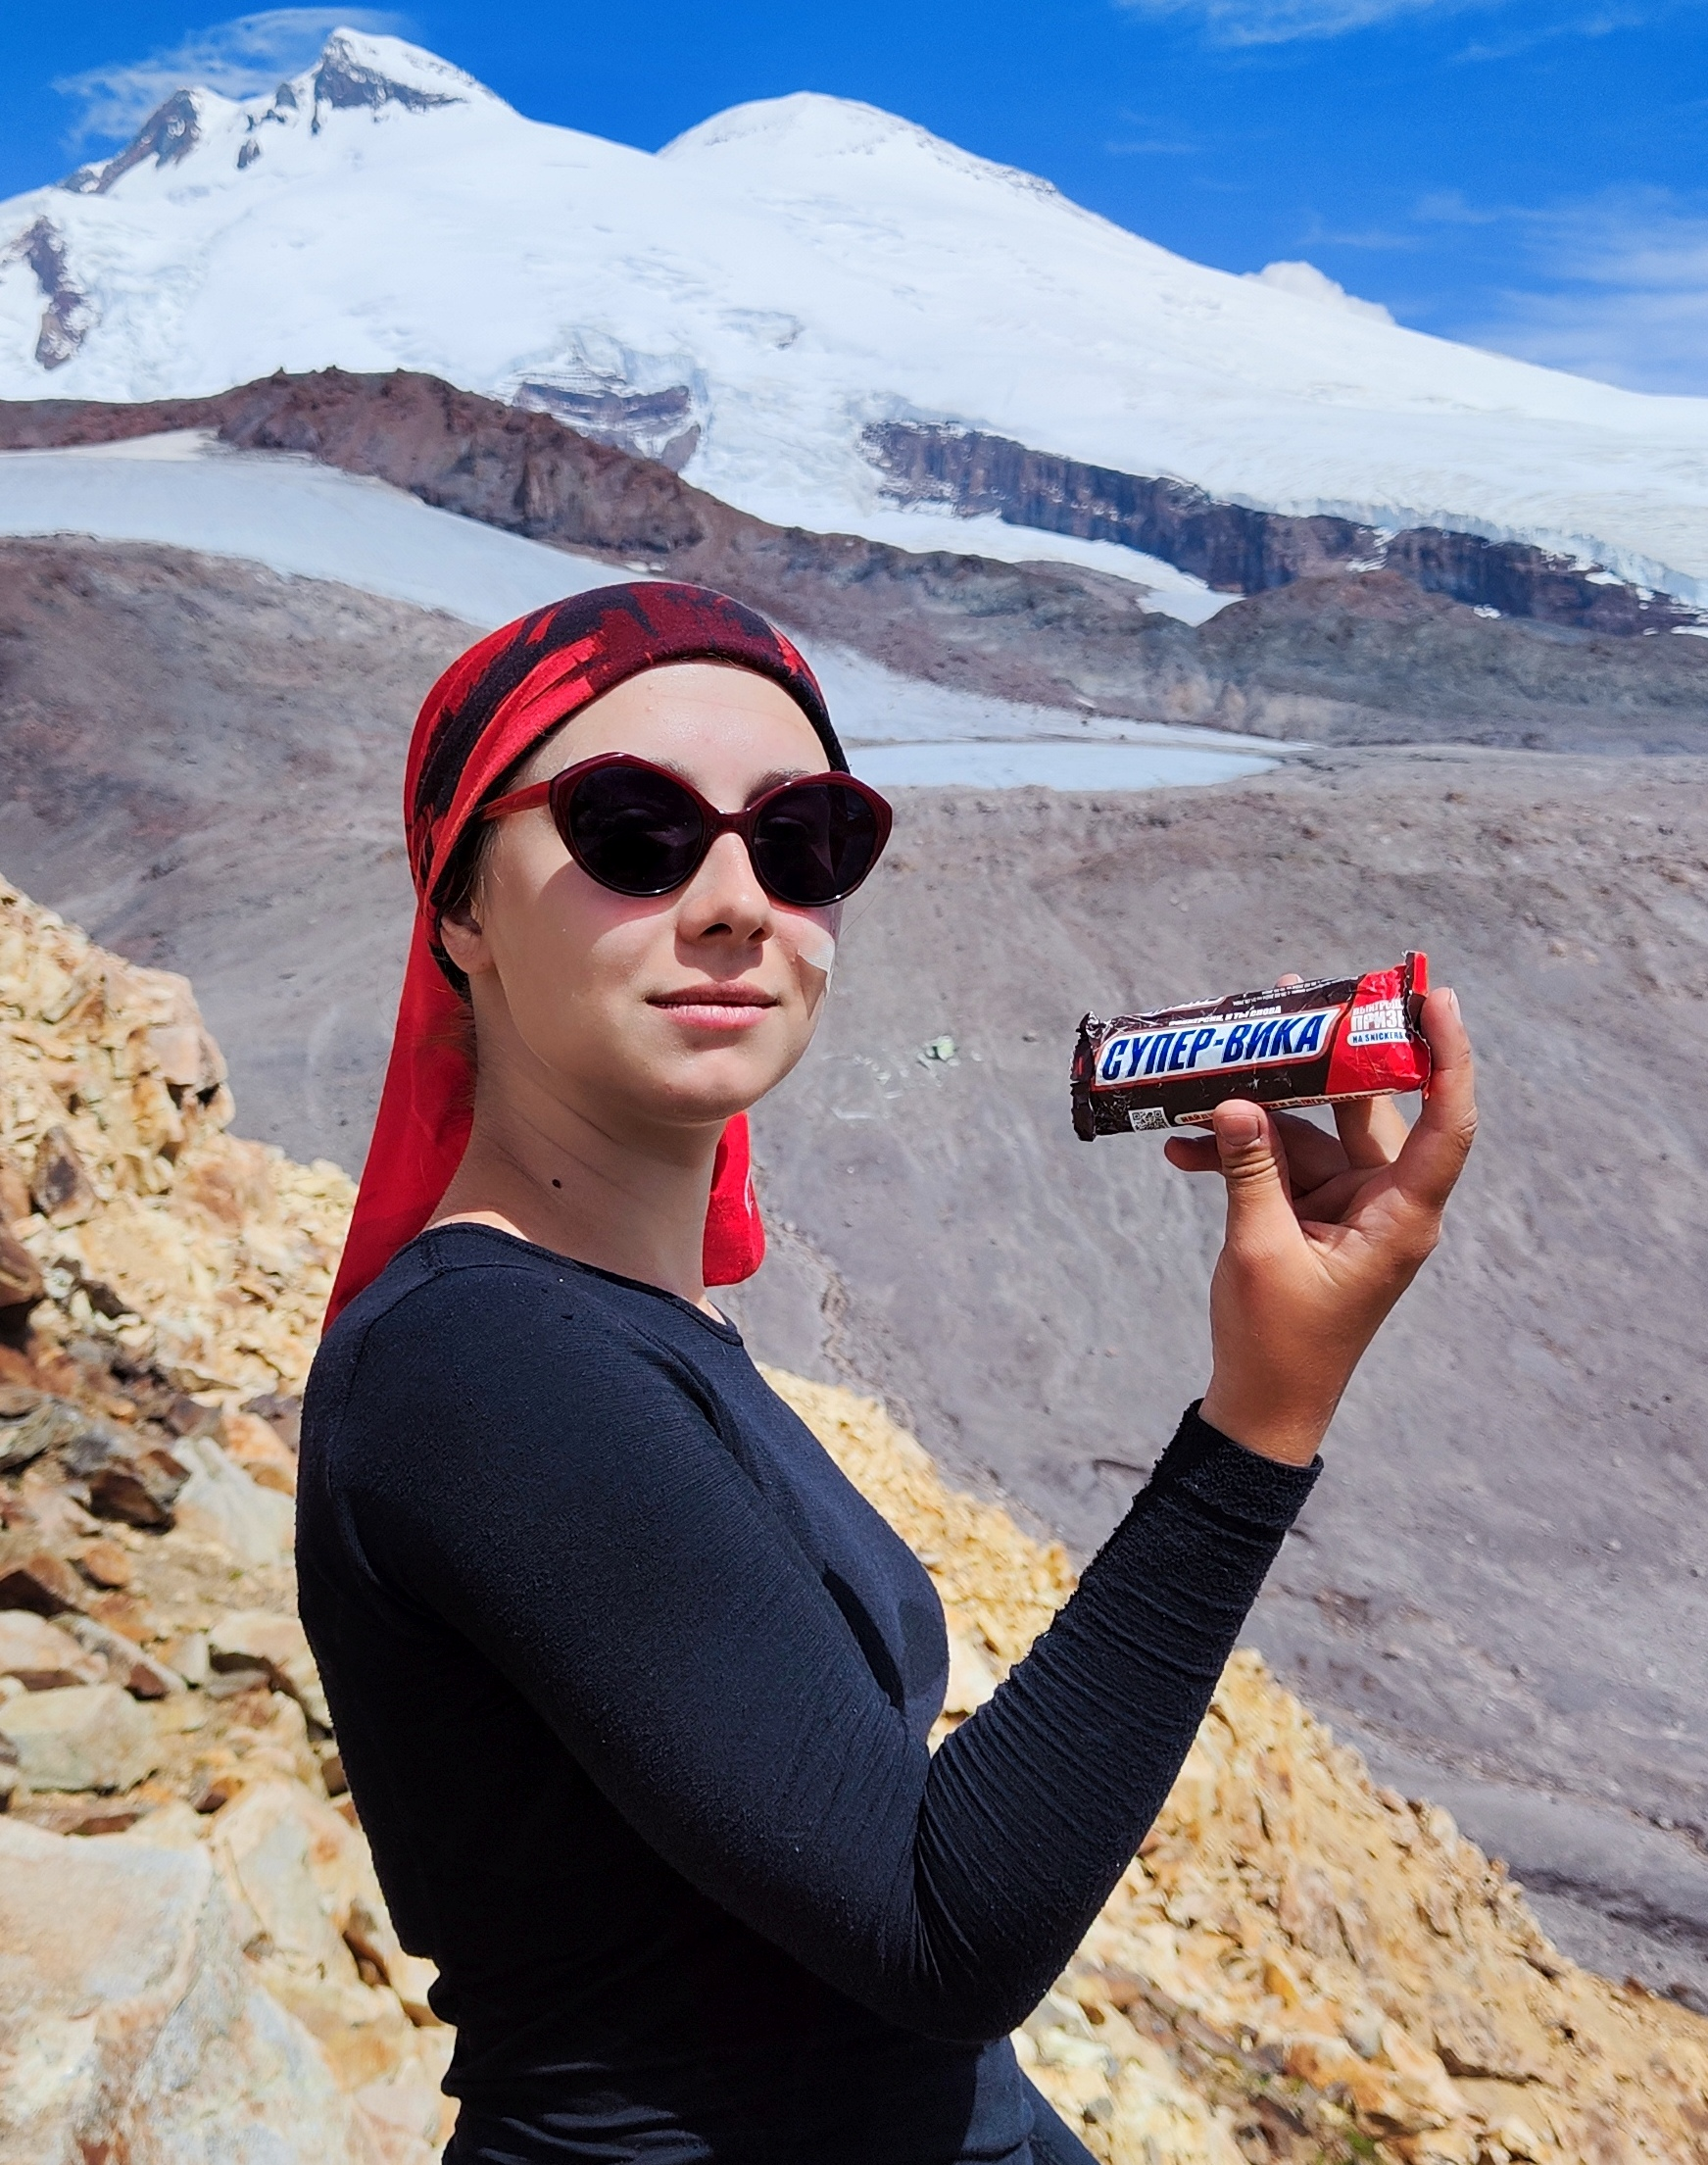
\includegraphics[width=0.99\linewidth]{../pics/portraits/vika}	&	Суровцева Виктория Павловна	&	2002	&	Снаряженец	&	1 ст.с. \\
		\hline
		8	&	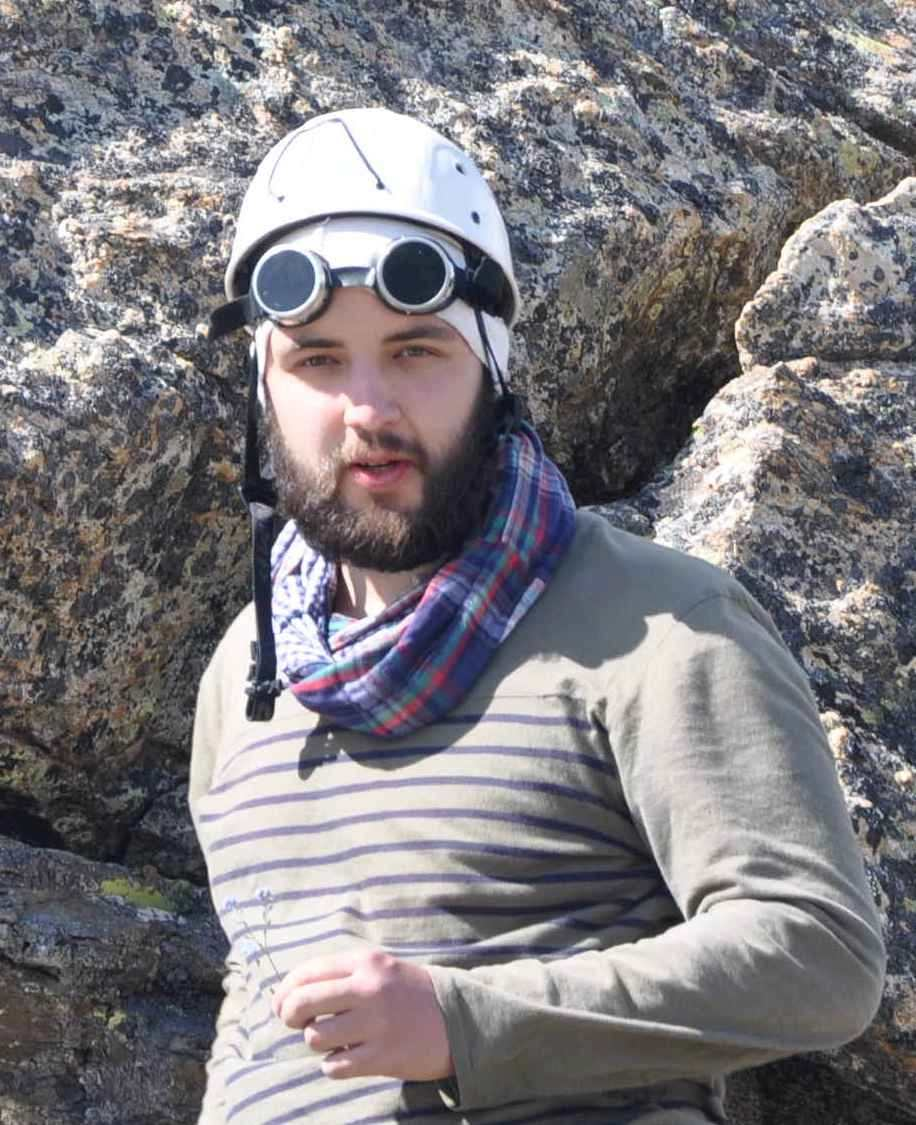
\includegraphics[width=0.99\linewidth]{../pics/portraits/gosha}		&	Корнилов Георгий Алексеевич	&	2003	&	Завхоз 1	&	1 ст.с. \\
		\hline
		9	&	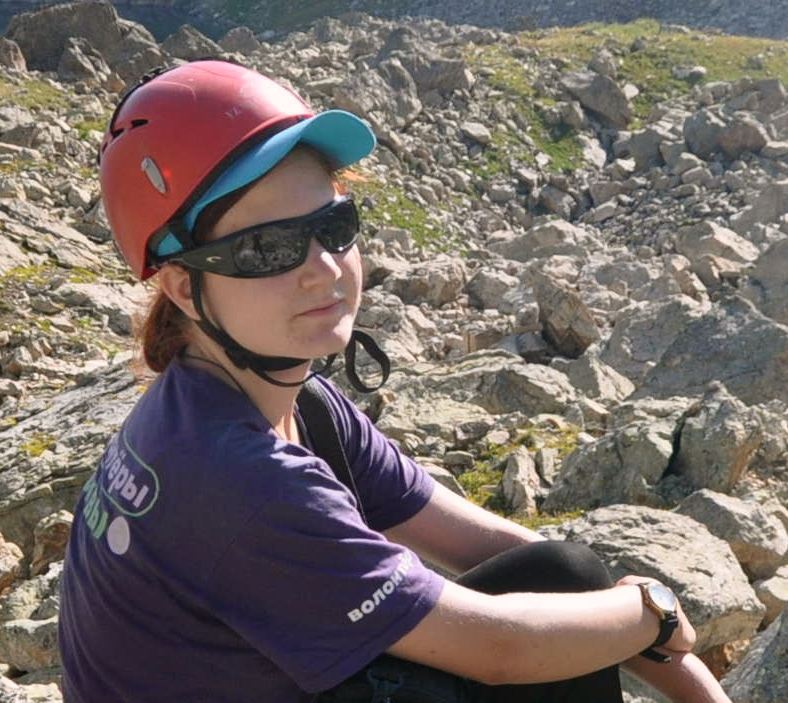
\includegraphics[width=0.99\linewidth]{../pics/portraits/masha}	&	Семено Мария Алексеевна	&	2006	&	Завхоз	2	&	1 ст.с. \\
		\hline
		10	&	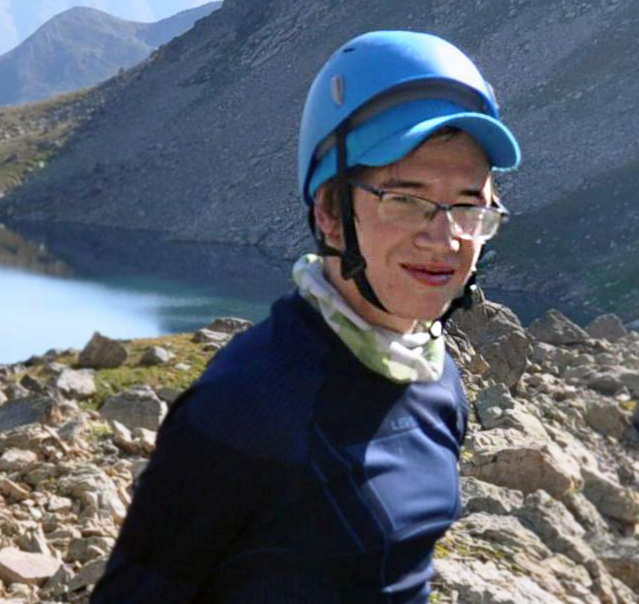
\includegraphics[width=0.99\linewidth]{../pics/portraits/dima_s}	&	Сингалевич Дмитрий Константинович	&	2004	&	Эколог	&	1 ст.с. \\
		\hline
		11	&	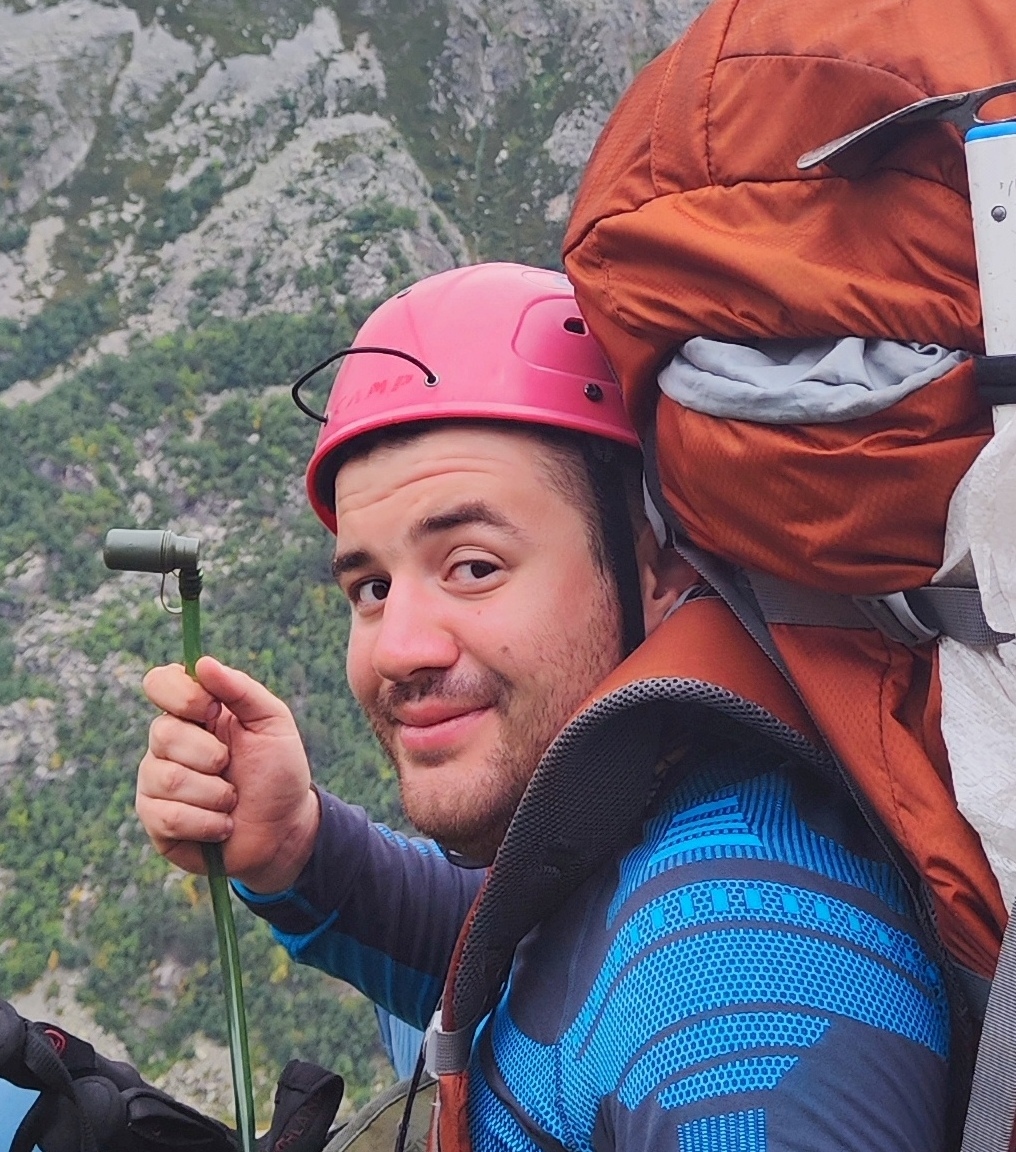
\includegraphics[width=0.99\linewidth]{../pics/portraits/ilya_sh}	&	Шалфеев Илья Андреевич	&	1997	&	Финансист	&	1 ст.с. \\
		\hline
		12	&	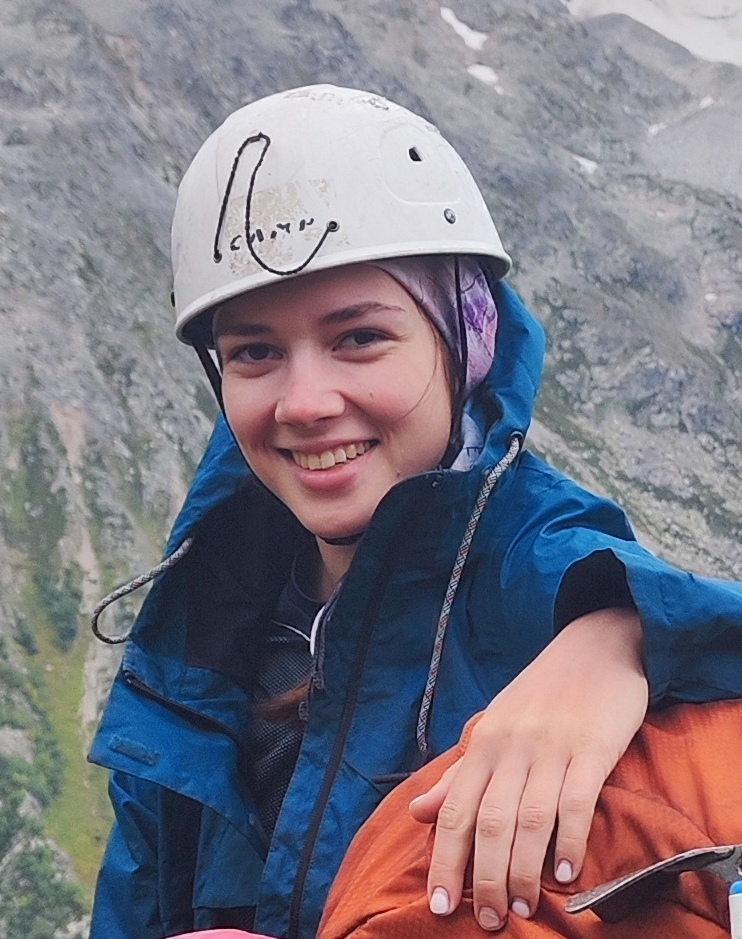
\includegraphics[width=0.99\linewidth]{../pics/portraits/dasha_m}	&	Мерзликина Дарья Сергеевна	&	2000	&	Реммастер	&	1 ст.с. \\
		\hline
		12$^\star$	&	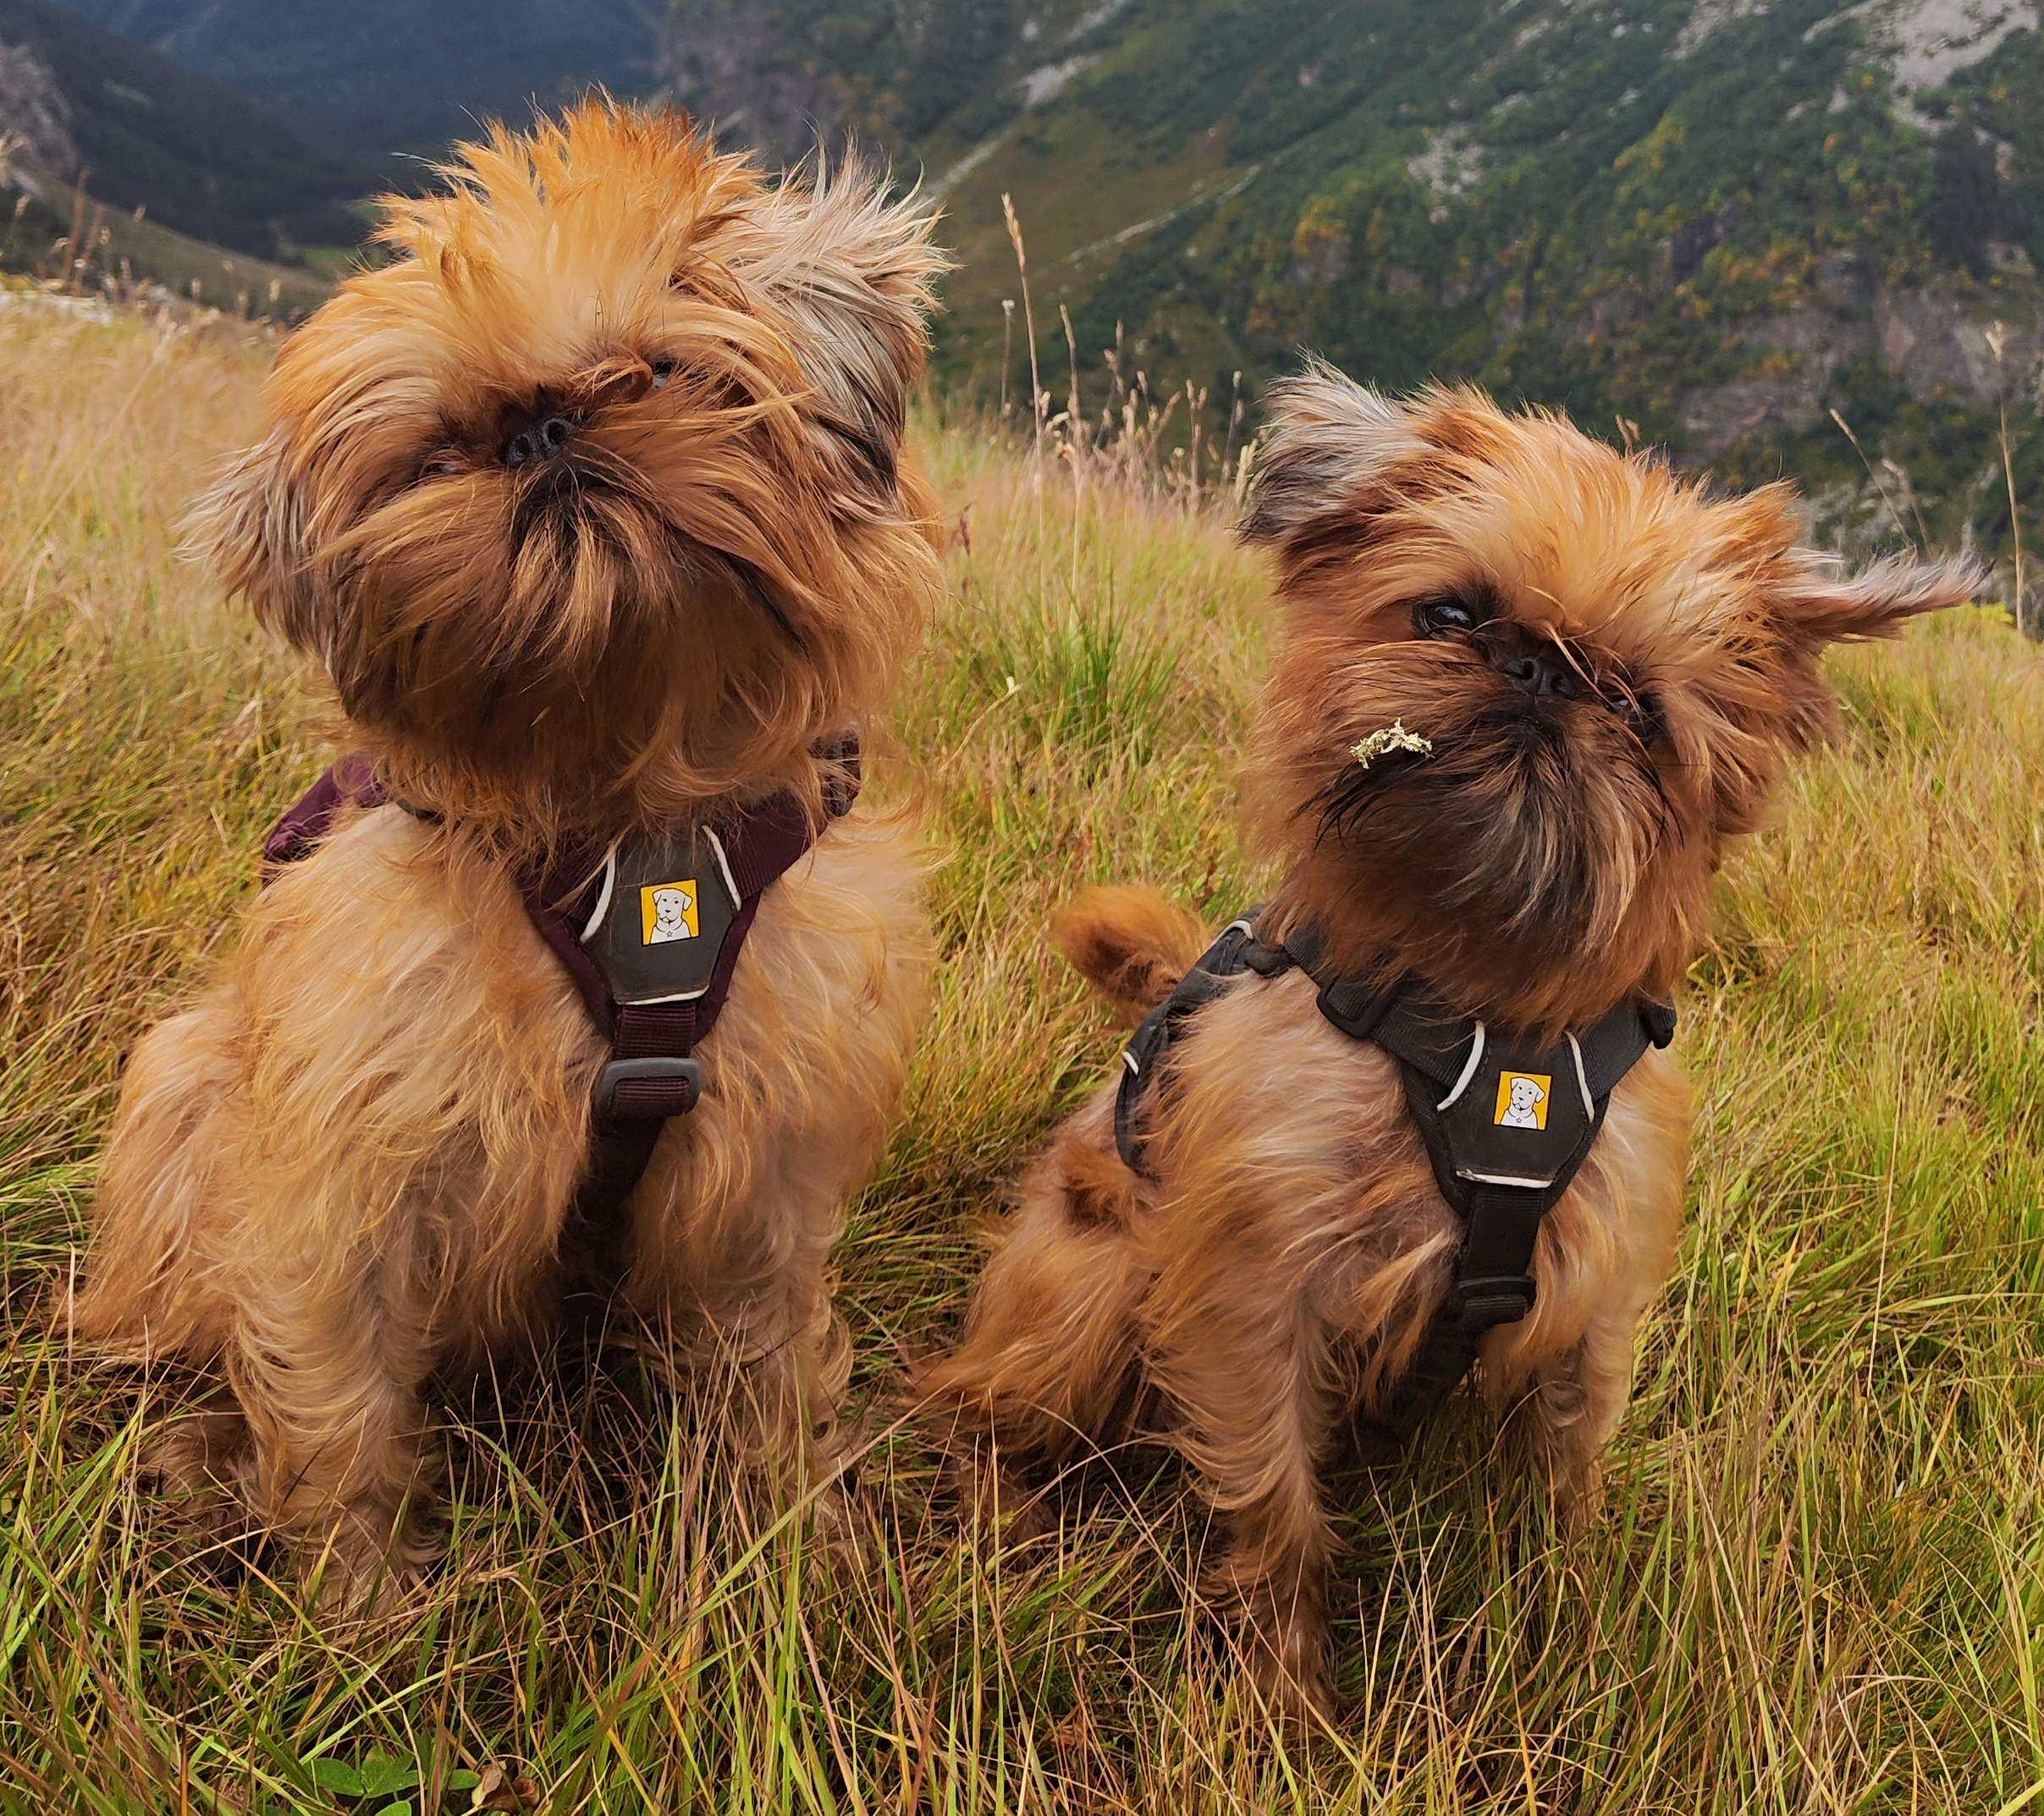
\includegraphics[width=0.8\linewidth]{../pics/portraits/yoshta_aina}	&	Йошта, Айна (брюссельские гриффоны)	&	2022	&	Талисманы команды	&	1 ст.с. \\
		\hline
	\end{tabular}%
	}
\end{table}

\newpage

\subsection{Географическое положение и туристские особенности района}
Район Гвандра, названный так по одноимённой вершине \textcolor{cyan}{Хде? в ГКХ N 43.20507° E 42.08093°},  расположен к западу от Эльбруса и пролегает \textcolor{teal}{(ад мора да мора...)} Район расположен в умеренном и субтропическом поясах с высотами, находящимися в диапазоне от \textcolor{cyan}{чего} до \textcolor{cyan}{чего}. Температура летом колеблется здесь от... до...; влажность — в диапазоне от... до.... Среди летних месяцев наибольшее количество осадков выпадает на июнь, наименьшее — на август. \textcolor{cyan}{(уточнять ли дополнительно про температуру в августе?)}. Согласно отчётам и отзывам руководителей, днём в конце июля – начале августа между 13 и 16 часами очень велика  вероятность мелкого моросящего дождя. Особенно это характерно для спуска с перевала Джалпаккол Северный.

Для перевалов категорий 1А в этом районе характерны, в основном, осыпные склоны, однако не исключены и снежные. Вблизи перевальных взлётов на некоторых перевалах также есть остатки старых ледников, но по состоянию на 2024 год большинство ледников  стаяло. 

Долины рек достаточно широкие, на высотах до 2000 м в основном лесистые. Лес состоит из ???; из ягод распространены малина, черника, шикша. 

Район легко доступен для транспорта: дороги подходят под... Вертолётные площадки есть ГДЕ? у погранцов епт! Из альплагерей здесь находятся Узункол, Глобус(это не альплагерь! ),... 

В качестве исторических, культурных и иных достопримечательностей можно, безусловно, назвать Эльбрус со всей имеющейся на нём туристической инфраструктурой — а также, из нетривиального, — руины чего-то (пока хз, чего именно) в долине р. Кубань. 

\clearpage